\documentclass[letterpaper,12pt,oneside,final]{book}
%%
%%  Template de mémoire de maîtrise ou thèse de doctorat.
%%  Normalement, il n'est pas nécessaire de modifier ce document
%%  sauf pour changer les noms des fichiers à inclure.
%%
%%  Version: 2014-10-28
%%
%%  Accepte les caractères accentués dans le document (UTF-8).
\usepackage[utf8]{inputenc}
%%
%% Support pour l'anglais et le français (français par défaut).
%\usepackage[cyr]{aeguill}
\usepackage{lmodern}      % Police de caractères plus complète et généralement indistinguable visuellement de la police standard de LaTeX (Computer Modern).
\usepackage[T1]{fontenc}  % Bon encodage des caractères pour qu'Acrobat Reader reconnaisse les accents et les ligatures telles que ffi.
\usepackage[english,frenchb]{babel} % le langage par défaut est le dernier de la liste, c'est-à-dire français
%%
%% Charge le module d'affichage graphique.
\usepackage{graphicx}
\usepackage{epstopdf}  % Permet d'utiliser des .eps avec pdfLaTeX.
%%
%% Recherche des images dans les répertoires.
\graphicspath{{./images/}{./dia/}{./gnuplot/}}
%%
%% Un float peut apparaître seulement après sa définition, jamais avant.
\usepackage{flafter,placeins}
%%
%% Utilisation de natbib pour les citations et la bibliographie.
\usepackage{natbib}
\bibliographystyle{dinat}
\citestyle{plainnat}
%%
%% Autres packages.
\usepackage{amsmath,color,soulutf8,longtable,colortbl,setspace,ifthen,xspace,url,pdflscape}
%%
%% Support des acronymes.
\usepackage[nolist]{acronym}
\onehalfspacing                % Interligne 1.5.
%%
%% Définition d'un style de page avec seulement le numéro de page à
%% droite. On s'assure aussi que le style de page par défaut soit
%% d'afficher le numéro de page en haut à droite.
\usepackage{fancyhdr}
\fancypagestyle{pagenumber}{\fancyhf{}\fancyhead[R]{\thepage}}
\renewcommand\headrulewidth{0pt}
\makeatletter
\let\ps@plain=\ps@pagenumber
\makeatother

\usepackage{stringstrings}
\newcommand\estVoyelle[1]{
    \pdfmatch icase{^[aeiuo].*}{#1}
}

%%
%% Module qui permet la création des bookmarks dans un fichier PDF.
%\usepackage[dvipdfm]{hyperref}
\usepackage{hyperref}
\usepackage{caption}  % Hyperlien vers la figure plutôt que son titre.
\makeatletter
\providecommand*{\toclevel@compteur}{0}
\makeatother
%%
%% Définitions spécifiques au format de rédaction de Poly.
\usepackage{MemoireThese}
%%
%% Définitions spécifiques à l'étudiant.
%% -----------------------------------
%% ---> A MODIFIER PAR L'ETUDIANT <---
%% -----------------------------------
%%
%% Commandes qui affichent le titre du document, le nom de l'auteur, etc.
\newcommand\monPays{république algérienne démocratique et populaire}
\newcommand\monUniversite{université m'hamed bougara de boumerdes}
\newcommand\monUnivAbbr{UMBB}
\newcommand\monFaculte{faculté des sciences de l'ingénieur}
\newcommand\monFacAbbr{FSI - exINGM}
\newcommand\monTitre{Titre de mon document}
\newcommand\monPrenom{Abdelhak}
\newcommand\monNom{Bougouffa}
\newcommand\monEmail{abougouffa@fedoraproject.org}
%\newcommand\monBinomePrenom{Anis} % Informations de binôme, lesser en commentaire si vous travailler en monôme
%\newcommand\monBinomeNom{Hocine}
%\newcommand\monBinomeEmail{hocine.anis.1992@gmail.com}
\newcommand\monDepartement{InfoTronique}
\newcommand\maDiscipline{systèmes informatiques distribués}
\newcommand\monDiplome{M}        % (M)aster/licence ou (D)octorat
\newcommand\anneeDepot{2017}
\newcommand\moisDepot{juin}
\newcommand\monSexe{M}           % "M" ou "F"
\newcommand\PageGarde{N}         % "O" ou "N"
\newcommand\AnnexesPresentes{O}  % "O" ou "N". Indique si le document comprend des annexes.
\newcommand\mesMotsClef{Liste,de,mot-clés,séparés,par,des,virgules}
%%
%%  DEFINITION DU JURY
%%
%%  Pour la définition du jury, les macros suivantes sont definies:
%%  \PresidentJury, \DirecteurRecherche, \CoDirecteurRecherche, \MembreJury, \MembreExterneJury
%%
%%  Toutes les macros prennent 4 paramètres: Sexe (M/F), Prénom, Nom, Titres
\newcommand\monJury{\PresidentJury{M}{prénom}{nom}{Ph.~D.}\\
\DirecteurRecherche{F}{prénom}{nom}{Ph.~D.}\\
\MembreJury{M}{prénom}{nom}{Prof.}}

\ifthenelse{\equal{\monDiplome}{M}}{
\newcommand\monSujet{Mémoire de master}
\newcommand\monDipl{Master}
}{
\newcommand\monSujet{Thèse de doctorat}
\newcommand\monDipl{Philosophi\ae{} Doctor}
}
%%
%% Informations qui sont stockées dans un fichier PDF.
\hypersetup{
  pdftitle={\monTitre},
  pdfsubject={\monSujet},
  pdfauthor={\monPrenom{} \monNom},
  pdfkeywords={\mesMotsClef},
  bookmarksnumbered,
  pdfstartview={FitV},
  hidelinks,
  linktoc=all
}
%%
%% Il y a un document par chapitre du mémoire.
%%
\begin{document}
%%
%% Page de titre du mémoire.
\frontmatter
% Compte optionellement la page de garde dans la pagination.
\ifthenelse{\equal{\PageGarde}{O}}{\addtocounter{page}{1}}{}
\thispagestyle{empty}%
\begin{center}%
\vspace*{\stretch{1}}
\MakeUppercase\monPays\\
\vspace*{\stretch{1}}
\MakeUppercase\monUniversite~(\monUnivAbbr)\\
\vspace*{\stretch{1}}
\begin{center}
\huge{\textsf{\monTitre}}\\
\end{center}
\vspace*{\stretch{1}}
\MakeUppercase{\monPrenom~\monNom} \ifdefined\monBinomeNom{\&~\MakeUppercase{\monBinomePrenom~\monBinomeNom}}\fi \\
DÉPARTEMENT D\ifthenelse{\estVoyelle{\monDepartement}=0}{E~}{'}\MakeUppercase{\monDepartement}\\
\MakeUppercase\monFaculte~(\monFacAbbr)\\
\vspace*{\stretch{1}}
\ifthenelse{\equal{\monDiplome}{M}}{MÉMOIRE PRÉSENTÉ}{THÈSE PRÉSENTÉE} EN VUE DE L'OBTENTION\\
DU DIPLÔME DE \MakeUppercase{\monDipl}\\
(\MakeUppercase{\maDiscipline})\\
\MakeUppercase{\moisDepot} \anneeDepot
\end{center}%
\vspace*{\stretch{1}}
\copyright~\monPrenom~\monNom\ifdefined\monBinomeNom{\&~\monBinomePrenom~\monBinomeNom}\fi, \anneeDepot.
%%
%% Identification des membres du jury.
%%
\newpage\thispagestyle{empty}%
\begin{center}%
\vspace*{\stretch{2}}
\MakeUppercase\monPays\\
\vspace*{\stretch{0.2}}
\rule{15cm}{0.03cm}\\
\vspace*{\stretch{0.2}}
\MakeUppercase\monUniversite~(\monUnivAbbr)\\
\vspace*{\stretch{0.2}}
\MakeUppercase\monFaculte~(\monFacAbbr)\\
\vspace*{\stretch{0.2}}
\rule{15cm}{0.03cm}\\
\vspace*{\stretch{2}}
Ce\ifthenelse{\equal{\monDiplome}{M}}{~mémoire intitulé}{tte thèse intitulée}:\\
\vspace*{\stretch{1}}
\MakeUppercase{\monTitre}\\
\vspace*{\stretch{2}}
\end{center}%
\begin{flushleft}
présenté\ifthenelse{\equal{\monDiplome}{M}}{}{e}
par:~\ul{\mbox{\MakeUppercase{\monNom} \monPrenom}}
\ifdefined\monEmail{\footnote{\texttt{\href{mailto:\monEmail}{\monEmail}}}}\fi
\ifdefined\monBinomeNom
{~\& \ul{\mbox{\MakeUppercase{\monBinomePrenom~\monBinomeNom}}}}\fi
\ifdefined\monBinomeEmail{\footnote{\texttt{\href{mailto:\monBinomeEmail}{\monBinomeEmail}}}}\fi\\
en vue de l'obtention du diplôme de:~\ul{\mbox{\monDipl}}\\
a été dûment accepté\ifthenelse{\equal{\monDiplome}{M}}{}{e} par le jury d'examen constitué de:\end{flushleft}
\vspace*{\stretch{0.5}}
\monJury
\vspace*{\stretch{2}}
%%
\pagestyle{pagenumber}%
%% Dédicace
%%
%% La dédicace est un hommage que l'auteur souhaite
%% rendre à une ou plusieurs personnes de son choix.
%%
\chapter*{DÉDICACE}\thispagestyle{headings}
\addcontentsline{toc}{compteur}{DÉDICACE}
\begin{flushright}
  \itshape
  À tous mes amis du labos,\\
  vous me manquerez\ldots
\end{flushright}
          % Dédicace du document.
% Remerciements
%
%   Grâce aux remerciements, l'auteur attire l'attention du lecteur
% sur l'aide que certaines personnes lui ont apportée, sur leurs
% conseils ou sur toute autre forme de contribution lors de la
% réalisation de son mémoire. Le cas échéant, c'est dans cette section
% que le candidat doit témoigner sa reconnaissance à son directeur de
% recherche, aux organismes dispensateurs de subventions ou aux
% entreprises qui lui ont accordé des bourses ou des fonds de
% recherche.
\chapter*{REMERCIEMENTS}\thispagestyle{headings}
\addcontentsline{toc}{compteur}{REMERCIEMENTS}
%
Texte.
     % Remerciements.
% Résumé du mémoire.
%
%   Le résumé est un bref exposé du sujet traité, des objectifs visés,
% des hypothèses émises, des méthodes expérimentales utilisées et de
% l'analyse des résultats obtenus. On y présente également les
% principales conclusions de la recherche ainsi que ses applications
% éventuelles. En général, un résumé ne dépasse pas quatre pages.
%
%   Le résumé doit donner une idée exacte du contenu du mémoire ou de la thèse. Ce ne
% peut pas être une simple énumération des parties du document, car il
% doit faire ressortir l'originalité de la recherche, son aspect
% créatif et sa contribution au développement de la technologie ou à
% l'avancement des connaissances en génie et en sciences appliquées.
% Un résumé ne doit jamais comporter de références ou de figures.
\chapter*{RÉSUMÉ}\thispagestyle{headings}
\addcontentsline{toc}{compteur}{RÉSUMÉ}

Le résumé est un bref exposé du sujet traité, des objectifs visés,
des hypothèses émises, des méthodes expérimentales utilisées et de
l'analyse des résultats obtenus. On y présente également les
principales conclusions de la recherche ainsi que ses applications
éventuelles. En général, un résumé ne dépasse pas quatre pages.

Le résumé doit donner une idée exacte du contenu du mémoire ou de la thèse. Ce ne
peut pas être une simple énumération des parties du document, car il
doit faire ressortir l'originalité de la recherche, son aspect
créatif et sa contribution au développement de la technologie ou à
l'avancement des connaissances en génie et en sciences appliquées.
Un résumé ne doit jamais comporter de références ou de figures.
      % Résumé du sujet en français.
% Abstract
%
%   Résumé de la recherche écrit en anglais sans être
% une traduction mot à mot du résumé écrit en français.

\chapter*{ABSTRACT}\thispagestyle{headings}
\addcontentsline{toc}{compteur}{ABSTRACT}
%
\begin{otherlanguage}{english}

Written in English, the abstract is a brief summary similar to the previous
section {\selectlanguage{frenchb}(Résumé)}.  However, this section is not a
word for word translation of the French.

\end{otherlanguage}
          % Résumé du sujet en anglais.

{\setlength{\parskip}{0pt}
%%
%% Table des matières.
\renewcommand\contentsname{TABLE DES MATIÈRES}
\tableofcontents
%%
%% Liste des tableaux.
\renewcommand\listtablename{LISTE DES TABLEAUX}
\listoftables
%%
%% Table des figures.
\renewcommand\listfigurename{LISTE DES FIGURES}
\listoffigures
%%
%% Liste des annexes au besoin.
}

% Liste des sigles et abbréviations
\newcommand\abbrevname{LISTE DES SIGLES ET ABRÉVIATIONS}
\chapter*{\abbrevname}
\addcontentsline{toc}{compteur}{\abbrevname}
\pagestyle{pagenumber}
%
\begin{acronym}
  \acro{IETF}{Internet Engineering Task Force}
  \acro{OSI}{Open Systems Interconnection}
\end{acronym}
%
\begin{longtable}{lp{5in}}
IETF       & Internet Engineering Task Force\\
OSI        & Open Systems Interconnection\\
\end{longtable}

       % Liste des sigles et abréviations.
\ifthenelse{\equal{\AnnexesPresentes}{O}}{\listofappendices}{}
\mainmatter
%   Dans l'introduction, on présente le problème étudié et les buts
% poursuivis. L'introduction permet de faire connaître le cadre de la
% recherche et d'en préciser le domaine d'application. Elle fournit
% les précisions nécessaires en ce qui concerne le contexte de
% réalisation de la recherche, l'approche envisagée, l'évolution de
% la réalisation. En fait, l'introduction présente au lecteur ce
% qu'il doit savoir pour comprendre la recherche et en connaître la
% portée.
\Chapter{INTRODUCTION}\label{sec:Introduction}  % 10-12 lignes pour introduire le sujet.
Texte en \emph{italique}, \textsc{petites majuscules}, mot \mbox{insécable}.\\
Texte \ul{souligné}, \hl{surligné}, \textbf{gras}.\\
Texte entre ``guillemets''.\\
Police \texttt{monospace}.\\
Un mot courant en réseautique mobile: n\oe{}ud\footnote{Note de bas de page.}.\\
L'objet RSVP \texttt{SENDER\_TEMPLATE}.\\
Nom d'un auteur: \citeauthor{RFC_IPv4}.\\
Une architecture 32~bits.\\
%%
%%  CONCEPTS DE BASE
%%
\section{Définitions et concepts de base}  % environ 2-3 pages
\begin{flushleft}
1\iere{} utilisation d'un acronyme: \ac{IETF}.\\
2\ieme{} utilisation d'un acronyme: \ac{IETF}.\\
Acronyme au long: \acl{IETF}.\\
\end{flushleft}

\subsection{Une sous-section}
Un URL: \href{http://www.polymtl.ca}{École Polytechnique de Montréal}.

\subsubsection{Une sous-sous-section}
Les besoins des flots de données peuvent être catégorisés selon
quatre paramètres importants \citep[voir][sect.\,5.4]{Tanenbaum} ou:
\begin{itemize}
\item la fiabilité (acheminement des données avec succès)~;
\item le délai de \mbox{bout-en-bout} de la source vers la destination~;
\item la variation du délai de \mbox{bout-en-bout} (\emph{jitter})~;
\item la bande passante requise (le débit des informations).
\end{itemize}

\paragraph{Le niveau paragraphe} est plus bas encore dans la hiérarchie\ldots
Une citation entre parenthèses \citep[voir][]{ART_ARTP}.
ou des citations entre parenthèses \citep[][]{nichols2010,PHD_HPMRSVP,ART_HMRSVP}.

\clearpage

%%
%% ELEMENTS DE LA PROBLEMATIQUE
%%
\section{Éléments de la problématique}  % environ 3 pages
La description de \mbox{l'en-tête} commun de RSVP est détaillée ci-dessous:\\
\begin{tabular}{p{1in}p{4.5in}}
&\\ % Ligne vide
\texttt{Ver}: & \texttt{4 bits}\\
          & Version du protocole. La version actuelle est~1.\\[5pt]
\texttt{Flags}: & \texttt{4 bits}\\
          & Aucun Flag n'est défini. L'émetteur doit (\textbf{MUST})
          mettre le champ à zéro et le récepteur doit (\textbf{MUST})
          ignorer ce champ.\\[5pt]
\texttt{Msg Type}: & \texttt{8 bits}\\
          & Type de message\\[5pt]
\texttt{Checksum}: & \texttt{16 bits}\\
          & Complément à un du complément à un de la somme des champs
          de \mbox{l'en-tête}, avec le champ Checksum à~0 pour des
          fins de calcul. La valeur~0 signifie qu'aucun Checksum n'a
          été transmis. Si le résultat du calcul du Checksum donne~0,
          la valeur 0xFFFF doit être stockée dans ce champ.\\[5pt]
\texttt{TTL}: & \texttt{8 bits}\\
          & Valeur originelle du champ \texttt{TTL} utilisée pour
          transmettre ce message.\\[5pt]
\texttt{Reserved}: & \texttt{8 bits}\\
          & Réservé pour usage futur. L'émetteur doit (\textbf{MUST})
          mettre le champ à zéro et le récepteur doit (\textbf{MUST})
          ignorer ce champ.\\[5pt]
\texttt{Length}: & \texttt{16 bits}\\
          & Longueur totale du message en octets, incluant
          \mbox{l'en-tête} commun et tous les objets de longueur
          variable.
\end{tabular}

\subsection{Autres types de structures de données}
L'énumération:
\begin{enumerate}
\item Un item~;
\item Un autre item.
\end{enumerate}


\subsection{Le protocole IPv6}
Voir la Figure~\ref{fig:IPv6} pour plus de détails. Le champs DSCP est
décrit dans le Tableau~\ref{tab:RangesDSCP}.

\begin{figure}[htb]
\centering
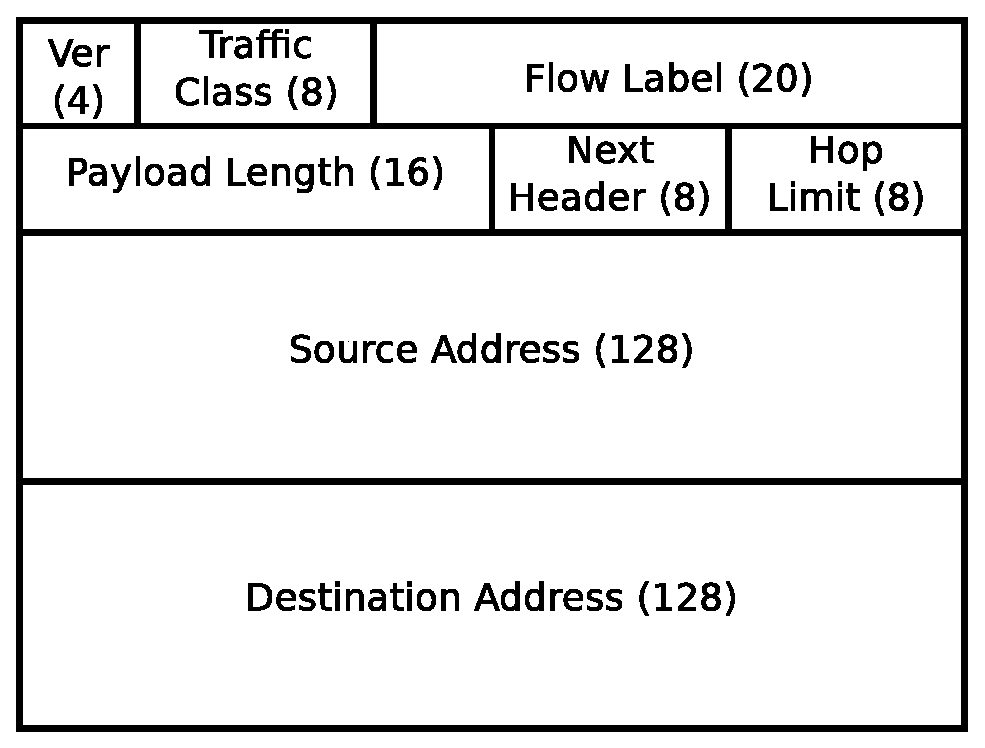
\includegraphics[width=4in]{IPv6_header}
\caption{L'en-tête IPv6}
\label{fig:IPv6}
\end{figure}

\begin{table}[ht]
\caption{Plages de valeurs pour le champ \texttt{DSCP}}
\centering
\begin{tabular}{|c|c|l|}
\hline\rowcolor[gray]{0.8}\color{black}
Plage & Valeurs & Règle d'assignation\\\hline
1 & xxxxx0 & Assignation par une norme de l'IANA\\\hline
2 & xxxx11 & Expérimentation/Usage local\\\hline
3 & xxxx01 & Expérimentation/Usage local (pourrait être jointe à la plage 1)\\\hline
\end{tabular}
\label{tab:RangesDSCP}
\end{table}

% On veut éviter que la figure et le tableau soient placés au-delà de la section courante.
\FloatBarrier


%%
%% OBJECTIFS DE RECHERCHE
%%
\section{Objectifs de recherche}  % 0.5 page
Les objectifs de la recherche sont de concevoir un algorithme $O(n)$.


%%
%% PLAN DU MEMOIRE
%%
\section{Plan du mémoire}  % 0.5 page
Un tableau:
\begin{table}[htbp]
  \centering
  \caption{Constantes et variables du modèle analytique}
  \begin{tabular}{|c|l|}
    \hline\rowcolor[gray]{0.8}\color{black}
    Symbole         & Description\\\hline
    $\lambda$       & Taux d'arrivée moyen des requêtes de réservation de ressources\\\hline
    $\frac{1}{\mu}$ & Durée moyenne d'une session\\\hline
    $C$             & Capacité d'une cellule (nombre de sessions supportées)\\\hline
    $v_{moy}$       & Vitesse moyenne des MN dans le réseau d'accès\\\hline
    $L$             & Longueur d'un côté d'une cellule carrée\\\hline
    $n$             & Nombre moyen de MN dans une cellule\\\hline
    $\rho$          & Charge d'une cellule\\\hline
    $P_b$           & Probabilité de blocage d'une requête de réservation\\\hline
    $P_f$           & Probabilité d'interruption forcée d'une session\\\hline
    $P_c$           & Probabilité de compléter une session avec succès\\\hline
    $\Delta{}T$     & Délai de transmission\\\hline
  \end{tabular}
  \label{tab:Definitions}
\end{table}

La formule d'\mbox{Erlang-B}:
\begin{equation}
  P_b = \frac{\frac{\rho^C}{C!}}{\sum\limits_{x=0}^{C}\frac{\rho^x}{x!}}
  \label{eq:Pblock}
\end{equation}

Une autre équation:
\begin{equation}
  \begin{split}
    P_c &= (1 - P_b) \times (1 -  P_f)^N\\
        &= (1 - P_b)^{N+1}
  \end{split}
  \label{eq:ProbComplete}
\end{equation}

Enfin, l'expression suivante indique le moment à partir duquel les
réservations de ressources sont en place:
\begin{equation}
  \Delta{}T_{init} =
  \begin{cases}
    2\Delta{}T_{E2E} & \Delta{}T_{wan} > (\Delta{}T_{rad} + \Delta{}T_{net})\\
    \Delta{}T_{E2E} + 3(\Delta{}T_{rad} + \Delta{}T_{net}) & \text{sinon}
  \end{cases}
  \label{eq:InitCost}
\end{equation}

\paragraph{Le taux de paquets perdus} correspond au nombre de paquets
éliminés à cause d'une erreur de \emph{checksum} à un n\oe{}ud
quelconque ou d'une situation de congestion. Le taux de paquets perdus
pour un chemin est déterminé de la façon suivante:
\begin{equation}
  \label{eq:genPLR}
  PLR_P = 1 - \prod_{i=1}^N(1 - PLR_i)
\end{equation}

Toutefois, si les taux d'erreurs sont très faibles, comme c'est
généralement le cas pour des liens optiques, on peut approximer
$PLR_P$ de façon à le transformer en un paramètre additif:
\begin{equation}
  \label{eq:approxPLR}
  \begin{split}
    PLR_{L_1 \oplus L_2} &= 1 - (1 - PLR_1)(1 - PLR_2)\\
    &= 1 - (1 - PLR_2 - PLR_1 + \underbrace{PLR_1
      \times PLR_2}_\text{négligeable})\qquad PLR_1 \ll 1,
    PLR_2 \ll 1\\
    &\approx PLR_1 + PLR_2
  \end{split}
\end{equation}

\clearpage

Une courbe:
\begin{figure}[htb]
\centering
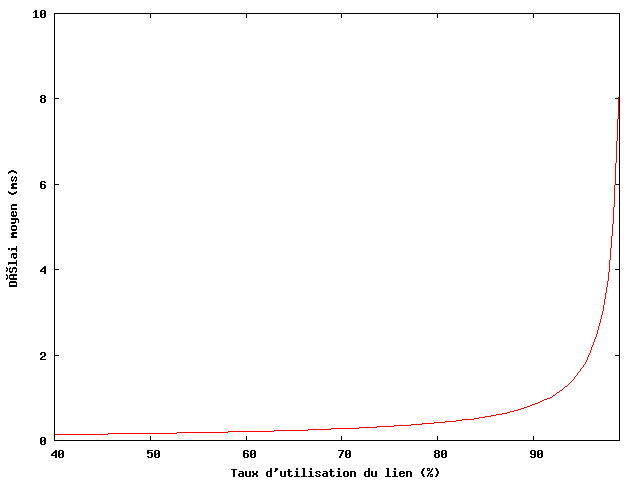
\includegraphics[width=5in]{LinkUsage}
\caption{Délai moyen en fonction du taux d'utilisation d'un lien}
\label{fig:LinkUse}
\end{figure}

\selectlanguage{english}
This paragraph is formatted by \LaTeX{} according to the standard rules of the
English language (\mbox{e.g.} hyphenation).
\selectlanguage{french}

L'arithmétique en virgule flottante peut entraîner des erreurs
d'approximation et il est important d'en être conscient
\citep[voir][]{Goldberg1991}.

De même, les calculs effectués sur une carte graphique (GPU) peuvent
introduire des erreurs d'approximation \citep{Benz2012, DSilva2012,
  Dabrowski2011, DeDinechin2011, DeFigueiredo2004, Filliatre2007,
  Fousse2007, Goubault2001, Goubault2008, Harder, Higham2002, Tanenbaum,
  Whitehead2011, mpmath, nichols2010, nvidia2012, Benz2012, Bao2013}.
       % Introduction au sujet de recherche.
\Chapter{REVUE DE LITTÉRATURE}\label{sec:RevLitt}
Texte.
  % Revue de littérature.
\Chapter{PREMIER THÈME}\label{sec:Theme1}
Texte.
             % Premier thème (Doctorat) ou "Détails de la Solution" (Maîtrise).
\Chapter{SECOND THÈME}\label{sec:Theme2}
Texte.
             % Second thème (Doctorat) ou "Résultats théoriques et expérimentaux" (Maîtrise).
\Chapter{TROISIÈME THÈME AVEC UN TITRE TRÈS LONG QUI S'ÉTEND SUR DEUX LIGNES}\label{sec:Theme3}

Lorem ipsum dolor sit amet, non faucibus ut, ante integer tristique odio
vitae turpis in. Euismod ullamcorper urna eget sollicitudin consectetuer,
dolor a. Ridiculus volutpat fusce, montes ipsum placerat, eu malesuada
maecenas a odio per, est pellentesque integer auctor sed ut sed, lectus
sodales orci ornare. Donec neque turpis vehicula. Duis vel sapien nec massa
lobortis nonummy. Feugiat ultrices urna mauris.

Potenti erat molestie ridiculus placerat, viverra ut felis porttitor,
rhoncus accumsan non, dui magna quam justo, ultrices massa ut phasellus
donec viverra mauris. Mauris a, dictumst risus a ornare velit nulla
ultricies, neque leo pellentesque, sit sed et suscipit excepteur
aenean. Venenatis sodales, odio nostra in id nobis scelerisque, venenatis
sociosqu gravida blandit orci pellentesque, tincidunt velit sed elementum
lacus pretium nunc, aenean vel dui id. Elit placerat id dui nunc mollis,
diam sapien porta, ipsam elit magna imperdiet amet, erat feugiat, et eros
morbi feugiat velit fringilla. Lacinia phasellus lacinia magna nunc sed, a
rhoncus, sem eget, dui aliquam sit sed leo beatae non, quisque justo
dignissim.

Torquent curabitur magnis nullam viverra scelerisque, per lacus pellentesque
vivamus, mauris aliquam sem lacus vivamus nullam porta. Vivamus donec
maecenas nunc orci massa, orci neque luctus leo non, mauris quis metus
sagittis. Voluptatibus gravida interdum. Magna duis nulla odio lacus fugiat
non. Magna fusce nunc, eget pellentesque nec. Imperdiet non magna
sollicitudin pellentesque, fusce erat interdum diam tellus vel, vitae
iaculis lectus varius suspendisse. Ac vel a in semper tellus, lobortis sed,
ipsum volutpat. Mauris a nunc aliquam metus nec, eu et id risus, diam
integer molestie suspendisse, sed wisi. Metus sed justo sodales sapien
molestie, suspendisse sem viverra ac proin, lorem luctus at tellus, velit mi
morbi orci in vestibulum, dignissim urna ornare id donec. Suspendisse non
enim euismod odio elit mauris, consectetuer pellentesque faucibus velit ante
lacinia sed.

Et dui erat. Wisi lorem eleifend cursus do donec, sed vel fermentum nec, a a
in pharetra. Ultricies risus, eget habitasse in, consectetuer metus in
auctor ac pellentesque curabitur, pulvinar aliquet eget. Mattis eget
venenatis dolor, nunc sem sed massa, urna scelerisque a magnis, neque elit
nec aliquam nonummy ac accusantium. Id vivamus nunc, erat justo tellus,
scelerisque habitasse accumsan tellus, pede sem vestibulum velit in et
eleifend. Nulla massa aenean integer dui. Suscipit nunc purus, rutrum velit,
mi torquent elementum in tincidunt. Maecenas nulla integer fringilla dapibus
tellus sit, enim amet magna eu erat, libero consectetuer nisl sapien, in
ultricies neque arcu sodales sagittis.

Lorem ipsum dolor sit amet, non faucibus ut, ante integer tristique odio
vitae turpis in. Euismod ullamcorper urna eget sollicitudin consectetuer,
dolor a. Ridiculus volutpat fusce, montes ipsum placerat, eu malesuada
maecenas a odio per, est pellentesque integer auctor sed ut sed, lectus
sodales orci ornare. Donec neque turpis vehicula. Duis vel sapien nec massa
lobortis nonummy. Feugiat ultrices urna mauris.

Potenti erat molestie ridiculus placerat, viverra ut felis porttitor,
rhoncus accumsan non, dui magna quam justo, ultrices massa ut phasellus
donec viverra mauris. Mauris a, dictumst risus a ornare velit nulla
ultricies, neque leo pellentesque, sit sed et suscipit excepteur
aenean. Venenatis sodales, odio nostra in id nobis scelerisque, venenatis
sociosqu gravida blandit orci pellentesque, tincidunt velit sed elementum
lacus pretium nunc, aenean vel dui id. Elit placerat id dui nunc mollis,
diam sapien porta, ipsam elit magna imperdiet amet, erat feugiat, et eros
morbi feugiat velit fringilla. Lacinia phasellus lacinia magna nunc sed, a
rhoncus, sem eget, dui aliquam sit sed leo beatae non, quisque justo
dignissim.

Torquent curabitur magnis nullam viverra scelerisque, per lacus pellentesque
vivamus, mauris aliquam sem lacus vivamus nullam porta. Vivamus donec
maecenas nunc orci massa, orci neque luctus leo non, mauris quis metus
sagittis. Voluptatibus gravida interdum. Magna duis nulla odio lacus fugiat
non. Magna fusce nunc, eget pellentesque nec. Imperdiet non magna
sollicitudin pellentesque, fusce erat interdum diam tellus vel, vitae
iaculis lectus varius suspendisse. Ac vel a in semper tellus, lobortis sed,
ipsum volutpat. Mauris a nunc aliquam metus nec, eu et id risus, diam
integer molestie suspendisse, sed wisi. Metus sed justo sodales sapien
molestie, suspendisse sem viverra ac proin, lorem luctus at tellus, velit mi
morbi orci in vestibulum, dignissim urna ornare id donec. Suspendisse non
enim euismod odio elit mauris, consectetuer pellentesque faucibus velit ante
lacinia sed.

Et dui erat. Wisi lorem eleifend cursus do donec, sed vel fermentum nec, a a
in pharetra. Ultricies risus, eget habitasse in, consectetuer metus in
auctor ac pellentesque curabitur, pulvinar aliquet eget. Mattis eget
venenatis dolor, nunc sem sed massa, urna scelerisque a magnis, neque elit
nec aliquam nonummy ac accusantium. Id vivamus nunc, erat justo tellus,
scelerisque habitasse accumsan tellus, pede sem vestibulum velit in et
eleifend. Nulla massa aenean integer dui. Suscipit nunc purus, rutrum velit,
mi torquent elementum in tincidunt. Maecenas nulla integer fringilla dapibus
tellus sit, enim amet magna eu erat, libero consectetuer nisl sapien, in
ultricies neque arcu sodales sagittis.

             % Troisième thème (Doctorat) ou effacez ce fichier si vous êtes à la Maîtrise.
\Chapter{CONCLUSION}\label{sec:Conclusion}
Texte.

%%
%%  SYNTHESE DES TRAVAUX
%%
\section{Synthèse des travaux}
Texte.

%%
%%  LIMITATIONS
%%
\section{Limitations de la solution proposée}\label{sec:Limitations}

%%
%%  AMELIORATIONS FUTURES
%%
\section{Améliorations futures}
Texte.
         % Conclusion.
%\backmatter
\renewcommand\bibname{RÉFÉRENCES}
\bibliography{Document}
%\bibliographystyle{dinat}  % Format de la bibliographie.
%\bibliographystyle{IEEEtranSN-francais}  % Format de la bibliographie.
%
\ifthenelse{\equal{\AnnexesPresentes}{O}}{
\appendix%
\newcommand{\Annexe}[1]{\annexe{#1}\setcounter{figure}{0}\setcounter{table}{0}\setcounter{footnote}{0}}%
%%
%%  Annexes.
%%
%%  Note: Ne pas modifier la ligne ci-dessous.
\addcontentsline{toc}{compteur}{ANNEXES}
%%
%%
%%  Toutes les annexes doivent être inclues dans ce document
%%  les unes à la suite des autres.
\Annexe{DÉMO}
Texte de l'annexe A\@. Remarquez que la phrase précédente se termine
par une lettre majuscule suivie d'un point. On indique explicitement
cette situation à \LaTeX{} afin que ce dernier ajuste correctement
l'espacement entre le point final de la phrase et le début de la
phrase suivante.


\begin{landscape}
\Annexe{ENCORE UNE ANNEXE}
Texte de l'annexe B\@ en mode «landscape».
\end{landscape}

\Annexe{UNE DERNIÈRE ANNEXE}
Texte de l'annexe C\@.
}{}
\end{document}
